\documentclass{article}
\usepackage{graphicx} % new way of doing eps files
\usepackage{listings} % nice code layout
\usepackage[usenames]{color} % color
\definecolor{listinggray}{gray}{0.9}
\definecolor{graphgray}{gray}{0.7}
\definecolor{ans}{rgb}{1,0,0}
\definecolor{blue}{rgb}{0,0,1}
% \Verilog{title}{label}{file}
\graphicspath{ {H:/ELC3338/Team8/CompOrg_Spring2018_S1_Team8/images/} }
\newcommand{\Verilog}[3]{
  \lstset{language=Verilog}
  \lstset{backgroundcolor=\color{listinggray},rulecolor=\color{blue}}
  \lstset{linewidth=\textwidth}
  \lstset{commentstyle=\textit, stringstyle=\upshape,showspaces=false}
  \lstset{frame=tb}
  \lstinputlisting[caption={#1},label={#2}]{#3}
}


\author{Matthew Carrano and Breana Leal}
\title{Lab 5: Control Unit and Sign Extender}

\begin{document}
\maketitle

\section{Simplified Report}
The control module uses a portion of the instruction data, the opcode field, as inputs to define which control signals to set. The set signals will determine which signals the processor will use. The Sign Extender module uses the address from the instruction code and outputs a 64 bit sign extended version. Using the expected results table, the module is verified.

\section{Code}
\Verilog{Verilog code for implementing the control module.}{code:adder}{../code/2_decode/control.v}



\Verilog{Verilog code for implementing the sign extender module.}{code:mux}{../code/2_decode/sign_extender.v}


\section{Testbench}

\Verilog{Verilog code for implementing the control testbench.}{code:adder}{../code/2_decode/control_test.v}


\Verilog{Verilog code for implementing the sign extender testbench.}{code:mux}{../code/2_decode/sign_ext_test.v}




\section{Simulation}

\begin{figure}[h]	
	\caption{Timing diagram for control module test.}
	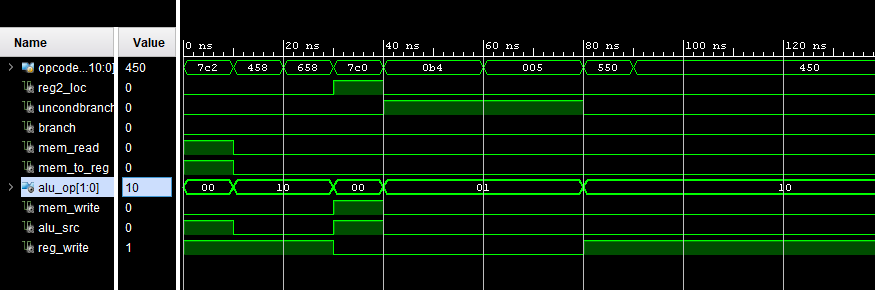
\includegraphics[width=\textwidth]{control_sim}
	
\end{figure}

\begin{figure}[h]	
	\caption{Timing diagram for sign extender module test.}
	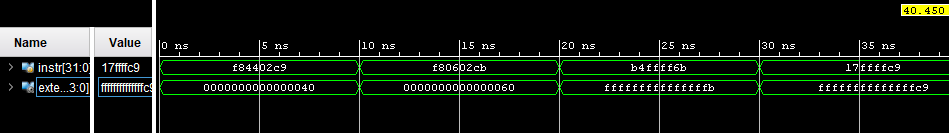
\includegraphics[width=\textwidth]{sign_ext_sim}
	\label{fig:fetchtest}
\end{figure}
\end{document} 